\documentclass[../document.tex]{subfiles}
\begin{document}
\section{Results}
In the section we show and evaluate the models results. We will start by presenting to the reader the networks score on each metric, then we will use the best models to predict the traversability of real world terrain. Finally, we will use handcrafted patches, for example a wall of a certain height in a specific position, to test the robustness of the network by trying to highlighting its behaviour.
\subsection{Experiment Setup}
\subsubsection{Hardware}
We run all the experiment on a Ubuntu 18.10  work station equipped with a Ryzen 2700x, a powerful CPU with 8 cores and 16 threads, and a NVIDIA 1080 GPU with 8GB of dedicated RAM.
\subsubsection{Dataset}
For the classification task, we select a threshold of $0.2$m on a time window, $\Delta t$, of two seconds to label the patches, meaning that a patch with an advancement less than $20$ centimeters is labeled as \emph{no traversable} and viceversa. This processed is explained in detail in the previous chapter. We minimise the binary Cross Entropy. 

While, for regression, we did not label the patch and directly regress on the advancement  minimising the Mean Square Error (MSE). 

Initially, to train the models in booth cases we first use Standard Gradient Descent with momentum set to $0.95$ and weight decay to $1e-4$ with an initial learning rate of $1e-3$ as was originally proposed to train residual network \cite{he2015deep}. However, we later utilize Leslie Smith's 1cycle policy \cite{1cycle} that allows us to trian the network faster and with an higher accuracy.
\subsubsection{Experimental validation}
We select as \emph{validation} ten percent of the training data. We remain to the reader that we store each run of \emph{Krock} as a \emph{.csv} file. So, to avoid any biases, we used completely different dataframes, meaning that train and validation sets are composed by non overlapping data from the simulations.
\todo[inline]{add more maps if we add them to the test set}
\subsubsection{Metrics}

\paragraph{Classification:} To evaluate the model's classification performance we used two metrics: \emph{accuracy} and \emph{AUC-ROC Curve}. Accuracy scores the number of correct predictions made by the network while AUC-ROC Curve represents degree or measure of separability, informally it tells how much model is capable of distinguishing between classes. For each experiment, we select the model with the higher AUC-ROC Curve during training to be evaluated on the test set.



\paragraph{Regression:} We used the Mean Square Error to evaluate the model's performance.
\subsection{Quantitative Results}
\subsubsection{Model selection}
We compared two different \emph{micro-resnet} and the \emph{vanilla} cnn from the previous Chapter. We evaluate those models using a time window of two second, a threshold of $20$cm and the data augmentation techniques described before. We run five experiments per architecture and we select the best performing network, the results are showed in the following table. 

\begin{table*}[h]
  \centering
  \ra{1.2}
  \begin{tabular}{@{}lcccc@{}}
  \toprule
   && Vanilla & \multicolumn{2}{c}{MicroResnetSE} \\
  \cline{3-5}
  && & $3\times 3$ stride $1$ & $7\times7$ stride $2$\\ 
  \cline{3-5}
  \multirow{2}{*}{AUC} & Top & 0.892 & 0.888 & \textbf{0.896}\\
   & Mean & \textbf{0.890} & 0.883 & 0.888\\
  \cline{1-5}
  Params & & 974,351 & 313,642 & 314,282  \\
  \bottomrule   
\end{tabular}
\caption{Model comparison on the test set.}
\end{table*}
\todo[inline]{Luca told me is better to split the models like Model1 and Model2 etc}

Based on this data We select \emph{micro-resnet} with squeeze and excitation and a starting convolution's kernel size of $7\times7$ with stride of $2$. This model has one third of the parameter of the origal model proposed by Chavez-Garcia et all \cite{omar2018traversability}. 

As proof of work, we also train the best network architecture, MicroResnetSE with a first convolution's kernel size of $7 \times 7$ and stride$=2$, with and without the Squeeze and Excitation operator.
\begin{table*}[h]
  \centering
  \ra{1.2}
  \begin{tabular}{@{}lccc@{}}
  \toprule
  &  MicroResnet$7\times7$ & MicroResnet$7\times7$-SE  & Improvement \\
  \cline{1-4}
   Top & 0.875 & \textbf{0.896} & $+0.021$ \\
   Mean & 0.867 & \textbf{0.888} & $+0.021$ \\
  \bottomrule   
\end{tabular}
\caption{AUC top value and mean value for MicroResnet with a fist convolution of $7\times7$ and stride $=2$ with and without the SE module. The improvement is the same.}
\end{table*}

\subsection{Final results}
The following table shows in deep the score of the best network for each dataset.
\begin{table*}[h]
    \centering
    \ra{1.2}
    \begin{tabular}{@{}llccccc@{}}
    \toprule
    % \multicolumn{8}{c}{Quantitative evaluation in simulation} \\
    \multicolumn{2}{c}{Dataset} && \multicolumn{2}{c}{micro-resnet} & Size & Resolution(cm/px) \\
    \cmidrule{1-2} \cmidrule{4-5}
    Type     &  Name  & Samples & ACC  &  AUC    & & \\
    \toprule
      \multirow{3}{*}{Synthetic}  & Training   & 429312 & - & - & & 2\\
      &  Valdiation   & 44032 &  95.2 \% &  0.961 & & 2 \\
      & Arc Rocks & 37273 &  85.5 \% &  0.888 & & 2 \\
      \cmidrule{2-7}
    \multirow{3}{*}{\makecell[l]{Real\\evaluation}} & Quarry & 36224 &  88.2 \%&  0.896& & 2\\
    & foo & TODO & & & & \\
    & baaa & TODO & & & & \\
    \bottomrule   
\end{tabular}
\caption{Final results on different datasets.}
\end{table*}
\todo[inline]{I have actually never talk about surf rocks}

Moreover, we would like to also show the different steps we made to reach this result. The following table shows the metric's score without any data-augmentation.
\todo[inline]{add result with and without data agu}
Adding dropout increases the results.
\todo[inline]{table with results}
With dropout plus coarse dropout.
\todo[inline]{table with results}
\subsection{Qualitative results}
\todo[inline]{\textbf{THIS PLOT IS OLD!}}
We qualitative evaluate the models in real world scenarios by computing the traversability probability for each map with different rotation. Specifically, we used a sliding window to extract the patches from the heightmaps and colour by blue the relative region with the corresponding traversability probability. A brighter colour yields an higher probability. For each map we show the traversability from bottom to top, top to bottom, left to right and right to left since those are the most human understandable.
We will start by showing the traversability probability on the \emph{Quarry} assuming \emph{Krock} is walking from bottom to top.
\todo[inline]{add quarry textures from bottom to top}
Thanks its special locomotion, \emph{Krock} can traverse the big slopes in the top part of them map while obliously it is stock by big bumps near the bottom as show in the next figures.
\begin{figure}[H]
\centering
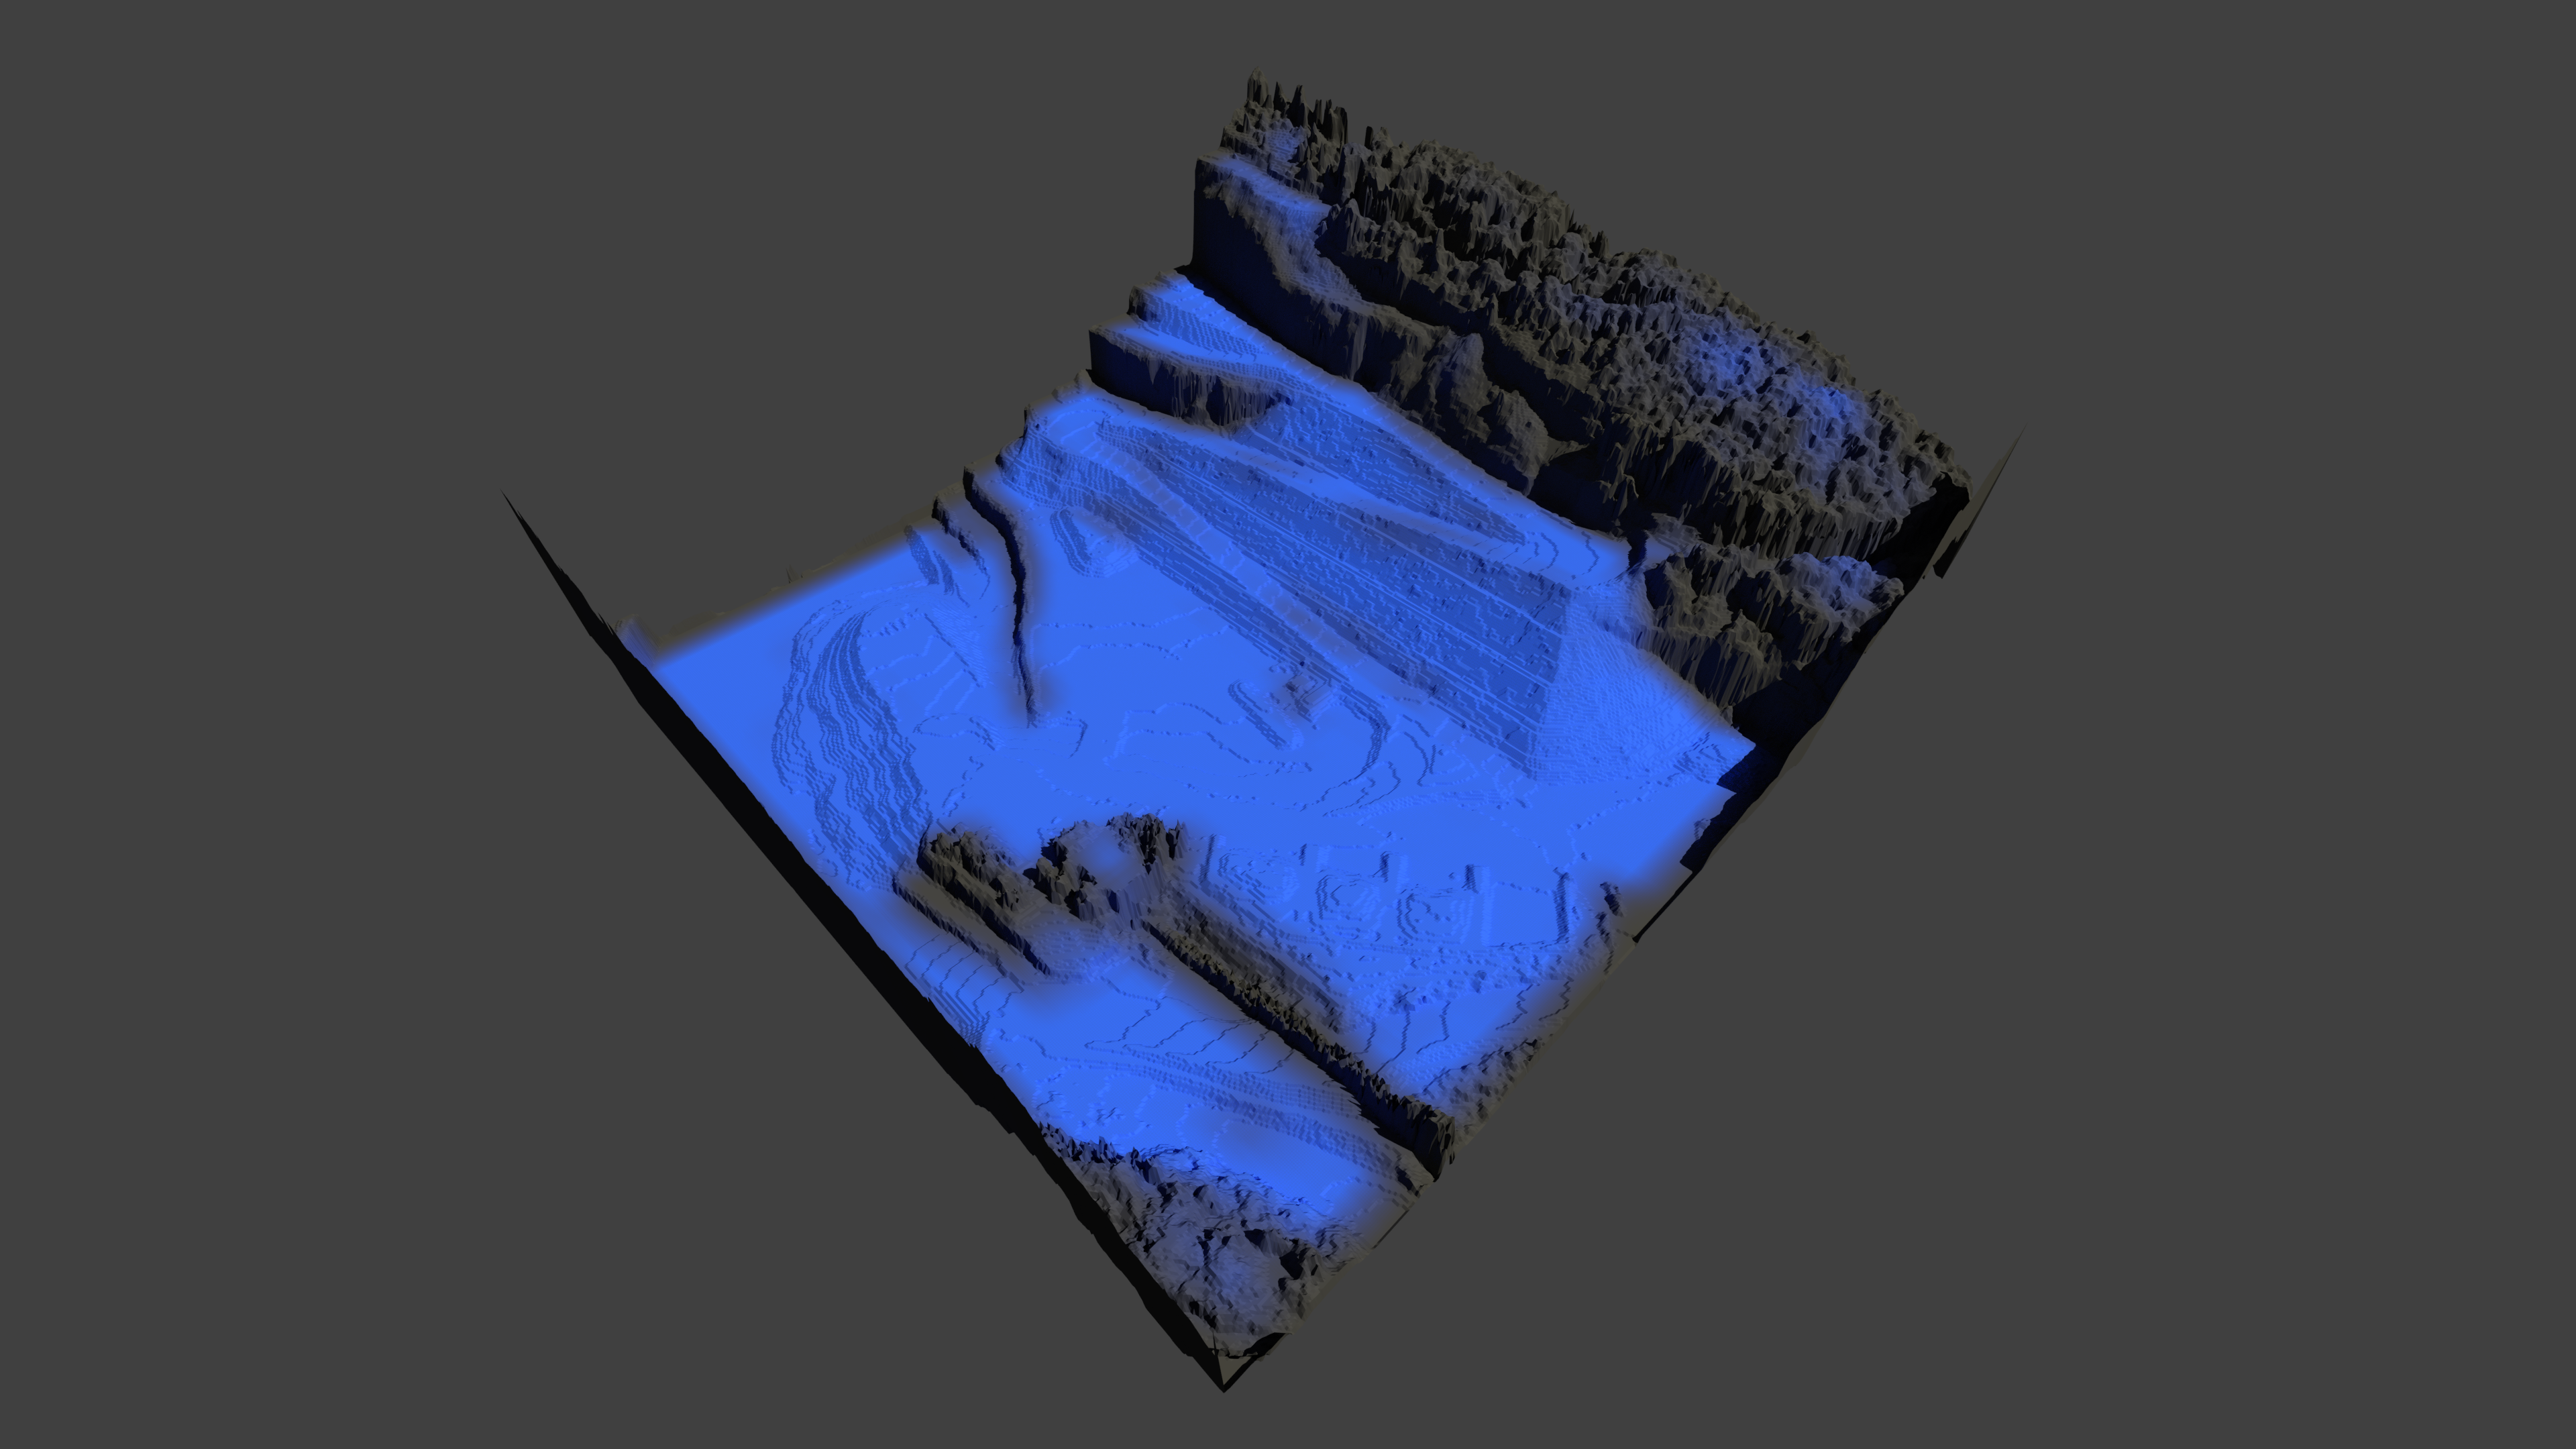
\includegraphics[width=\linewidth]{../img/4/traversability/quarry/querry-big-10-270.png}
\end{figure}
\todo[inline]{add figure of krock traversing the big slopes and getting stop near the bottom}
To convince the reader that those slopes can be traverse, we run \emph{Krock} on them directly from the simulator.
\todo[inline]{image of one extracted patch from quarry and one run on the simulator} 

\end{document}